%%%%%%%%%%%%%%%%%%%%%%%%%%%%%%%%%%%%%%%%%
% University/School Laboratory Report
% LaTeX Template
% Version 3.1 (25/3/14)
%
% This template has been downloaded from:
% http://www.LaTeXTemplates.com
%
% Original author:
% Linux and Unix Users Group at Virginia Tech Wiki 
% (https://vtluug.org/wiki/Example_LaTeX_chem_lab_report)
%
% License:
% CC BY-NC-SA 3.0 (http://creativecommons.org/licenses/by-nc-sa/3.0/)
%
%%%%%%%%%%%%%%%%%%%%%%%%%%%%%%%%%%%%%%%%%

%----------------------------------------------------------------------------------------
%	PACKAGES AND DOCUMENT CONFIGURATIONS
%----------------------------------------------------------------------------------------

\documentclass{article}

\usepackage{polski}
\usepackage[utf8]{inputenc}
\usepackage{booktabs}
\usepackage{multirow}
\usepackage{caption}

\usepackage[version=3]{mhchem} % Package for chemical equation typesetting
\usepackage{siunitx} % Provides the \SI{}{} and \si{} command for typesetting SI units
\usepackage{graphicx} % Required for the inclusion of images
\usepackage{natbib} % Required to change bibliography style to APA
\usepackage{amsmath} % Required for some math elements 

\setlength\parindent{0pt} % Removes all indentation from paragraphs

\renewcommand{\labelenumi}{\alph{enumi}.} % Make numbering in the enumerate environment by letter rather than number (e.g. section 6)
\usepackage{colortbl}

%\usepackage{times} % Uncomment to use the Times New Roman font

%----------------------------------------------------------------------------------------
%	DOCUMENT INFORMATION
%----------------------------------------------------------------------------------------

\title{Ćwiczenie nr 71: Dyfrakcja światła na szczelinie pojedynczej i podwójnej} % Title

\author{Rafał \textsc{Grabiański} i Zbigniew \textsc{Królikowski}} % Author name

\date{\today} % Date for the report

\addtolength{\oddsidemargin}{-.875in}
\addtolength{\evensidemargin}{-.875in}
\addtolength{\textwidth}{1.75in}
\addtolength{\topmargin}{-.875in}
\addtolength{\textheight}{1.75in}

\begin{document}

% Please add the following required packages to your document preamble:
% \usepackage{booktabs}
\begin{table}[h]
\begin{tabular}{@{}llllll@{}}
\toprule
\begin{tabular}[c]{@{}l@{}}Wydział:\\ \\ WIEiT\end{tabular}                                    & \multicolumn{2}{l}{\begin{tabular}[c]{@{}l@{}}Imię i nazwisko:\\ Rafał Grabiański\\ Zbigniew Królikowski\end{tabular}}                & \begin{tabular}[c]{@{}l@{}}Rok:\\ \\ II\end{tabular}            & \begin{tabular}[c]{@{}l@{}}Grupa:\\ \\ 7\end{tabular}              & \begin{tabular}[c]{@{}l@{}}Zespół:\\ \\ 7\end{tabular} \\ \midrule
\multicolumn{1}{|c|}{\begin{tabular}[c]{@{}c@{}}PRACOWNIA\\ FIZYCZNA\\ WFiIS AGH\end{tabular}} & \multicolumn{4}{l|}{Temat: Dyfrakcja światła na szczelinie pojedynczej i podwójnej}                                                                                                                                                                                                                                                  & \multicolumn{1}{l|}{Nr ćwiczenia: 71}                     \\ \midrule
\begin{tabular}[c]{@{}l@{}}Data wykonania:\\ \\ \\ 25.11.2014\end{tabular}                     & \begin{tabular}[c]{@{}l@{}}Data oddania:\\ \\ \\ 2.12.2014\end{tabular} & \begin{tabular}[c]{@{}l@{}}Zwrot do poprawy:\\ \\ \\ .\end{tabular} & \begin{tabular}[c]{@{}l@{}}Data oddania:\\ \\ \\ .\end{tabular} & \begin{tabular}[c]{@{}l@{}}Data zaliczenia:\\ \\ \\ .\end{tabular} & OCENA:                                                  \\ \bottomrule
\end{tabular}
\end{table}

%\maketitle % Insert the title, author and date

% If you wish to include an abstract, uncomment the lines below


%----------------------------------------------------------------------------------------
%	SECTION 1 - CEL ĆWICZENIA
%----------------------------------------------------------------------------------------

\section{Cel ćwiczenia}

Celem ćwiczenia było wyznaczenie rozkładu natężenia światła laserowego dla obrazu dyfrakcyjnego powstałego dla pojedynczej i układu dwóch szczelin. Za pomocą wykonanych pomiarów mieliśmy wyznaczyć szerokość szczeliny.


% If you have more than one objective, uncomment the below:
%\begin{description}
%\item[First Objective] \hfill \\
%Objective 1 text
%\item[Second Objective] \hfill \\
%Objective 2 text
%\end{description}


 


%----------------------------------------------------------------------------------------
%	SECTION 4
%----------------------------------------------------------------------------------------
\section{Wyniki pomiarów}

\begin{table}[h!tbp]
\centering
\scalebox{1}{
\begin{tabular}{|r|r|r|r|r|r|r|r|r|r|}
\hline
\multicolumn{1}{|l|}{\textbf{X [mm]}} & \multicolumn{1}{l|}{I [j.u.]} & \multicolumn{1}{l|}{\textbf{x [mm]}} & \multicolumn{1}{l|}{I [j.u.]} & \multicolumn{1}{l|}{\textbf{x [mm]}} & \multicolumn{1}{l|}{I [j.u.]} & \multicolumn{1}{l|}{\textbf{x [mm]}} & \multicolumn{1}{l|}{I [j.u.]} & \multicolumn{1}{l|}{\textbf{x [mm]}} & \multicolumn{1}{l|}{I [j.u.]} \\ \hline
-9.4 & 0.00 & -5.4 & 1.90 & -1.4 & 29.90 & 2.6 & 17.5 & 6.6 & -0.1 \\ \hline
-9.2 & 0.00 & -5.2 & 2.00 & -1.2 & 30.50 & 2.8 & 9.1 & 6.8 & -0.2 \\ \hline
-9 & 0.00 & -5 & 2.10 & -1 & 49.70 & 3 & 4.8 & 7 & -0.1 \\ \hline
-8.8 & 0.10 & -4.8 & 1.70 & -0.8 & 77.30 & 3.2 & 2.8 & 7.2 & 0 \\ \hline
-8.6 & 0.20 & -4.6 & 1.30 & -0.6 & 130 & 3.4 & 1.4 & 7.4 & 0.2 \\ \hline
-8.4 & 0.30 & -4.4 & 1.50 & -0.4 & 175 & 3.6 & 0.7 & 7.6 & 0.3 \\ \hline
-8.2 & 0.30 & -4.2 & 1.60 & -0.2 & 210 & 3.8 & 0.3 & 7.8 & 0.6 \\ \hline
-8 & 0.20 & -4 & 1.90 & 0 & 223 & 4 & 0.1 & 8 & 0.8 \\ \hline
-7.8 & 0.10 & -3.8 & 2.50 & 0.2 & 219 & 4.2 & 0.2 & 8.2 & 0.8 \\ \hline
-7.6 & 0.20 & -3.6 & 3.50 & 0.4 & 189 & 4.4 & 0.6 & 8.4 & 0.7 \\ \hline
-7.4 & 0.30 & -3.4 & 4.10 & 0.6 & 148 & 4.6 & 1.4 & 8.6 & 0.4 \\ \hline
-7.2 & 0.50 & -3.2 & 4.70 & 0.8 & 105 & 4.8 & 0.3 & 8.8 & 0.3 \\ \hline
-7 & 0.60 & -3 & 6.70 & 1 & 70 & 5 & 3.9 & 9 & 0.2 \\ \hline
-6.8 & 0.70 & -2.8 & 8.90 & 1.2 & 55.3 & 5.2 & 4.4 & 9.2 & 0.1 \\ \hline
-6.6 & 0.80 & -2.6 & 14.20 & 1.4 & 43.3 & 5.4 & 3.9 & 9.4 & 0.1 \\ \hline
-6.4 & 0.70 & -2.4 & 18.30 & 1.6 & 41.5 & 5.6 & 2.8 & 9.6 & 0.1 \\ \hline
-6.2 & 0.80 & -2.2 & 20.70 & 1.8 & 40.8 & 5.8 & 1.6 & 9.8 & 0 \\ \hline
-6 & 0.90 & -2 & 24.90 & 2 & 38.8 & 6 & 0.9 & 10 & 0 \\ \hline
-5.8 & 1.10 & -1.8 & 25.80 & 2.2 & 36.6 & 6.2 & 0.3 & 10.2 & 0 \\ \hline
-5.6 & 1.70 & -1.6 & 27.80 & 2.4 & 26.8 & 6.4 & 0 & \multicolumn{1}{l|}{} & \multicolumn{1}{l|}{} \\ \hline
\end{tabular}}
\label{}
\caption{Wyniki pomiarów natężenia światła dla dwóch szczelin}
\end{table}

\begin{table}[h!tbp]
\centering
\begin{tabular}{|r|r|r|r|r|r|r|r|r|r|}
\hline
\multicolumn{1}{|l|}{x [mm]} & \multicolumn{1}{l|}{I [j.u.]} & \multicolumn{1}{l|}{x [mm]} & \multicolumn{1}{l|}{I [j.u.]} & \multicolumn{1}{l|}{x [mm]} & \multicolumn{1}{l|}{I [j.u.]} & \multicolumn{1}{l|}{x [mm]} & \multicolumn{1}{l|}{I [j.u.]} & \multicolumn{1}{l|}{x [mm]} & \multicolumn{1}{l|}{I [j.u.]} \\ \hline
-22.4 & -3 & -14.2 & -2 & -6 & 26 & 2.2 & 386 & 10.2 & 9 \\ \hline
-22.2 & -3 & -14 & -1 & -5.8 & 37 & 2.4 & 352 & 10.4 & 7 \\ \hline
-22 & -3 & -13.8 & -1 & -5.6 & 62 & 2.6 & 310 & 10.6 & 5 \\ \hline
-21.8 & -3 & -13.6 & -1 & -5.4 & 77 & 2.8 & 269 & 10.8 & 4 \\ \hline
-21.6 & -3 & -13.4 & -1 & -5.2 & 91 & 3 & 247 & 11 & 3 \\ \hline
-21.4 & -3 & -13.2 & 0 & -5 & 101 & 3.2 & 222 & 11.2 & 3 \\ \hline
-21.2 & -3 & -13 & 0 & -4.8 & 132 & 3.4 & 186 & 11.4 & 2 \\ \hline
-21 & -3 & -12.8 & 0 & -4.6 & 174 & 3.6 & 155 & 11.6 & 0 \\ \hline
-20.8 & -2 & -12.6 & 0 & -4.4 & 194 & 3.8 & 123 & 11.8 & 0 \\ \hline
-20.6 & -2 & -12.4 & 0 & -4.2 & 218 & 4 & 106 & 12 & -1 \\ \hline
-20.4 & -2 & -12.2 & 0 & -4 & 228 & 4.2 & 88 & 12.2 & -2 \\ \hline
-20.2 & -2 & -12 & 0 & -3.8 & 273 & 4.4 & 68 & 12.4 & -2 \\ \hline
-20 & -2 & -11.8 & 0 & -3.6 & 328 & 4.6 & 48 & 12.6 & -2 \\ \hline
-19.8 & -2 & -11.6 & 1 & -3.4 & 348 & 4.8 & 32 & 12.8 & -2 \\ \hline
-19.6 & -2 & -11.4 & 1 & -3.2 & 356 & 5 & 24 & 13 & -2 \\ \hline
-19.4 & -2 & -11.2 & 3 & -3 & 376 & 5.2 & 16 & 13.2 & -2 \\ \hline
-19.2 & -2 & -11 & 5 & -2.8 & 381 & 5.4 & 9 & 13.4 & -2 \\ \hline
-19 & -2 & -10.8 & 5 & -2.6 & 426 & 5.6 & 4 & 13.6 & -2 \\ \hline
-18.8 & -2 & -10.6 & 7 & -2.4 & 477 & 5.8 & 1 & 13.8 & -2 \\ \hline
-18.6 & -2 & -10.4 & 8 & -2.2 & 489 & 6 & 0 & 14 & -2 \\ \hline
-18.4 & -2 & -10.2 & 8 & -2 & 498 & 6.2 & -1 & 14.2 & -2 \\ \hline
-18.2 & -2 & -10 & 9 & -1.8 & 499 & 6.4 & -2 & 14.4 & -1 \\ \hline
-18 & -2 & -9.8 & 12 & -1.6 & 523 & 6.6 & -2 & 14.6 & -1 \\ \hline
-17.8 & -2 & -9.6 & 11 & -1.4 & 523 & 6.8 & -1 & 14.8 & -1 \\ \hline
-17.6 & -2 & -9.4 & 10 & -1.2 & 552 & 7 & 0 & 15 & -1 \\ \hline
-17.4 & -2 & -9.2 & 9 & -1 & 563 & 7.2 & 1 & 15.2 & 0 \\ \hline
-17.2 & -2 & -9 & 7 & -0.8 & 563 & 7.4 & 3 & 15.4 & 0 \\ \hline
-17 & -2 & -8.8 & 5 & -0.6 & 564 & 7.6 & 4 & 15.6 & -1 \\ \hline
-16.8 & -1 & -8.6 & 4 & -0.4 & 582 & 7.8 & 5 & 15.8 & -1 \\ \hline
-16.6 & -1 & -8.4 & 3 & -0.2 & 589 & 8 & 7 & 16 & -1 \\ \hline
-16.4 & -1 & -8.2 & 2 & 0 & 593 & 8.2 & 9 & 16.2 & 0 \\ \hline
-16.2 & -1 & -8 & 1 & 0.2 & 588 & 8.4 & 10 & 16.4 & -1 \\ \hline
-16 & -1 & -7.8 & 0 & 0.4 & 573 & 8.6 & 11 & 16.6 & -2 \\ \hline
-15.8 & -1 & -7.6 & -1 & 0.6 & 577 & 8.8 & 11 & 16.8 & -2 \\ \hline
-15.6 & 0 & -7.4 & -2 & 0.8 & 559 & 9 & 12 & 17 & -2 \\ \hline
-15.4 & 0 & -7.2 & -1 & 1 & 548 & 9.2 & 13 & 17.2 & -2 \\ \hline
-15.2 & 0 & -7 & 0 & 1.2 & 531 & 9.4 & 12 & 17.4 & -2 \\ \hline
-15 & -1 & -6.8 & 2 & 1.4 & 506 & 9.6 & 11 & 17.6 & -2 \\ \hline
-14.8 & -1 & -6.6 & 5 & 1.6 & 473 & 9.8 & 9 & 17.8 & -2 \\ \hline
-14.6 & -2 & -6.4 & 9 & 1.8 & 433 & 10 & 9 & 18 & -2 \\ \hline
-14.4 & -2 & -6.2 & 13 & 2 & 414 & \multicolumn{1}{l|}{} & \multicolumn{1}{l|}{} & \multicolumn{1}{l|}{} & \multicolumn{1}{l|}{} \\ \hline
\end{tabular}
\caption{Wyniki pomiarów natężenia światła dla jednej szczeliny}
\label{}
\end{table}


\clearpage

%----------------------------------------------------------------------------------------
%	SECTION 5 - WYNIKI
%----------------------------------------------------------------------------------------

\section{Opracowanie wyników}

\begin{table}[htbp]
\centering
\scalebox{0.8}{
\begin{tabular}{|c|r|r|r|r|}
\hline
\textbf{Numer maksimum} & \textbf{Położenie z lewej [mm]} & \multicolumn{1}{c|}{\textbf{Położenie z prawej [mm]}} & \multicolumn{1}{c|}{\textbf{$x_{sr}$}} & \multicolumn{1}{c|}{\textbf{Obliczona odległość d}} \\ \hline
\textbf{1 minimum} & -7.40 & 6.40 & 6.90 & 9.19E-005 \\ \hline
\textbf{1 maksimum boczne} & -9.80 & 9.20 & 9.50 & 1.00E-004 \\ \hline
\textbf{2 minimum} & -14.40 & 13.20 & 13.80 & 9.19E-005 \\ \hline
\textbf{2 maksimum boczne} & -15.40 & 15.20 & 15.30 & 1.04E-004 \\ \hline
\end{tabular}}
\caption{Położenia maksimów i minimów oraz obliczona szerokość d dla szczeliny pojedynczej}
\label{}
\end{table}

\begin{table}[htbp]
\centering
\begin{tabular}{|c|c|c|c|c|}
\hline
\textbf{Element obrazu dyfrakcyjnego} & \textbf{$I_{l}$[j. u.]} & \textbf{$I_{p}$[j. u.]} & \textbf{I względne dośw.                          } & \textbf{I względne teor.} \\ \hline
\textbf{1 maksimum boczne} & 12 & 13 & 0.021 & 0.045 \\ \hline
\textbf{2 maksimum boczne} & 0 & 0 & 0.000 & 0.016 \\ \hline
\end{tabular}
\caption{Natężenie światła dla maksimów w jednostkach umownych dla szczeliny pojedynczej}
\label{}
\end{table}

\subsection{Pojedyncza szczelina}
\subsubsection{Wykres zależności natężenia światła I od położenia detektora x}

\begin{figure}[h]
	\centering
	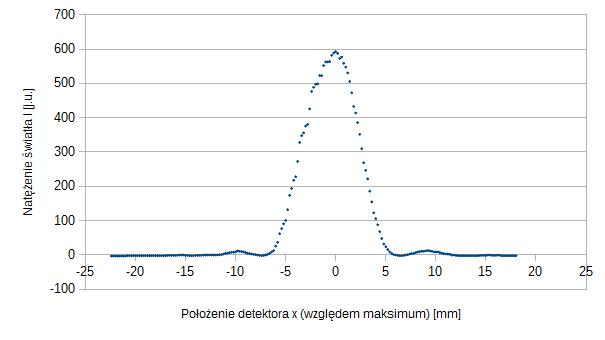
\includegraphics[scale=0.8]{ch01a}
	\caption{Wykres zależności natężenia światła I [j.u.], a położeniem detektora x [mm] dla szczeliny pojedynczej (we współrzędnych zwykłych)}
\end{figure}

\clearpage

\begin{figure}[h]
	\centering
	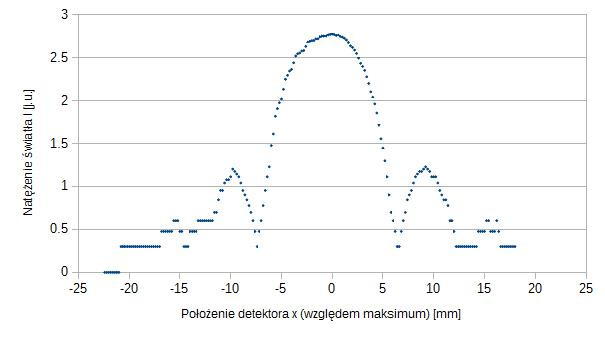
\includegraphics[scale=0.8]{ch02a}
	\caption{Wykres zależności natężenia światła I [j.u.], a położeniem detektora x [mm] dla szczeliny pojedynczej - wykres ze znormalizowaną i zlogarytmowaną osią pionową}
\end{figure}

\subsubsection{Odczytanie położeń minimów i maksimów bocznych}
Na podstawie uzyskanych danych uzupełniliśmy tabelę i wyliczyliśmy średnie współrzędne minimów i maksimów. Wyniki zamieściliśmy w tabeli 3.

\subsubsection{Wyznaczenie szerokości szczeliny}
Mając do dyspozycji wzory:
\begin{equation}
x_{min} = m \frac{\lambda L}{d}
\end{equation}
\begin{equation}
x_{max} = (m+\frac{1}{2}) \frac{\lambda L}{d}
\end{equation}

Na tej podstawie dla m = 1 wyliczamy szerokość szczeliny d jako:
\begin{equation}
d = \frac{\lambda L}{x_{min}}
\end{equation}
\begin{equation}
d = \frac{3}{2} \frac{\lambda L}{x_{max}}
\end{equation}
I analogicznie dla minimów i maksimów drugiego rzędu (tam za m podstawiamy 2).

Podstawiając uzyskane wyniki i przyjmując za $\lambda = 650 nm$ otrzymujemy d = $9.47 \cdot 10^{-5} m$ i odchylenie standardowe u(d) = $2.74  \cdot 10^{-6} m$
\subsubsection{Stosunek natężeń prążków bocznych do światła w maksimum}
Tu korzystamy ze wzoru:
\begin{equation}
	\frac{I(x_{max})}{I_{0}} = \frac{1}{\pi^{2}(m+\frac{1}{2})^{2}}
\end{equation}
Wyniki wstawiamy do tabeli 4.

\subsection{Podwójna szczelina}
\subsubsection{Wykres zależności natężenia światła I od położenia detektora x}
\begin{figure}[h!]
	\centering
	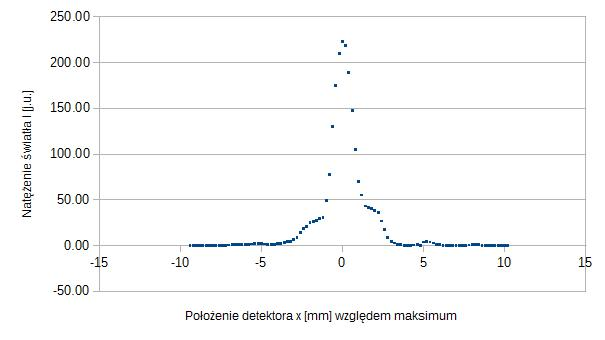
\includegraphics[scale=0.65]{ch03}
	\caption{Wykres zależności natężenia światła I [j.u.], a położeniem detektora x [mm] dla szczeliny pojedynczej (we współrzędnych zwykłych)}
\end{figure}
\begin{figure}[h!]
	\centering
	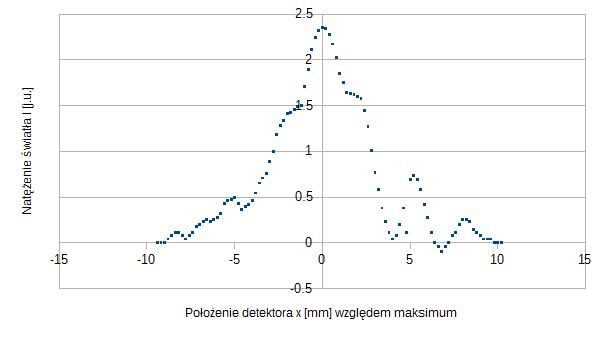
\includegraphics[scale=0.65]{ch04}
	\caption{Wykres zależności natężenia światła I [j.u.], a położeniem detektora x [mm] dla szczeliny pojedynczej (we współrzędnych zwykłych)}
\end{figure}
Numeracji dokonaliśmy odręcznie na sprawozdaniu.
\subsubsection{Odczytanie położeń minimów i maksimów bocznych i wyznaczenie odległości między szczelinami}
Postępując w podobny do pierwszego przypadku sposób, odczytujemy położenia maksimów i minimów. Obliczamy wartość średnią oraz  odległość między szczelinami d. Wyniki umieszczone w tabeli. Oczywiście wartość d liczymy teraz tak, że:
\begin{equation}
x_{max} = m \frac{\lambda L}{d}
\end{equation}
\begin{equation}
x_{min} = (m+\frac{1}{2}) \frac{\lambda L}{d}
\end{equation}
Wyniki umieszciliśmy w tabeli:
\begin{table}[htbp]
\centering
\begin{tabular}{|r|r|r|r|r|}
\hline
\multicolumn{1}{|c|}{\textbf{Nr maksimum}} & \multicolumn{1}{c|}{\textbf{$x_{l}$[mm]}} & \multicolumn{1}{c|}{\textbf{$x_{p}$ [mm]}} & \multicolumn{1}{c|}{\textbf{x [mm]}} & \multicolumn{1}{c|}{\textbf{Odległość d [mm]}} \\ \hline
1 & -1.6 & 2 & 1.80 & $3.5 \cdot 10^{-4}$ \\ \hline
2 & -5.00 & 5.20 & 5.10 & $2.5 \cdot 10^{-4}$ \\ \hline
3 & -8.40 & 8.40 & 8.40E+000 & $2.3 \cdot 10^{-4}$ \\ \hline
\end{tabular}
\caption{Wyznaczone położenia maksimów dla obrazu interferencyjnego dwóch szczelin.}
\label{}
\end{table}

\subsubsection{Wartość średnia d i niepewność u(d)}
Otrzymaliśmy $d = 3.0 \cdot 10^{-4} m$ oraz $u(d) = 4.2 \cdot 10^{-5} m$
\subsubsection{Wyznaczenie stosunku $I_{min}$ do $I_{max}$}
Nasze $I_{max}$ to 223 j.u. a $I_{min}$ 0.1. Czyli nasz współczynnik $\frac{I_{min}}{I_{max}} = 4.5*10^{-4}$ co jest bliskie zeru.


%----------------------------------------------------------------------------------------
%	SECTION 6
%----------------------------------------------------------------------------------------
\section{Wnioski}

Wyniki z doświadczenia korelowały z matematycznym opisem rozkładu natężenia światła na ekranie.

Otrzymana szerokość szczeliny w pierwszym doświadczeniu: $d = 9.47 \cdot 10^{-5}$ m co przy $u(d)= 2.74 \cdot 10^{-6}$ m i przyjęciu $k=2$ sprawia, że mieści się w przedziale razem z prawidziwym d = 0.1 mm.

Otrzymana odległość pomiędzy szczelinami w drugim doświadczeniu wynosi: $d = 3.01 \cdot 10^{-4}$ przy niepewności $4.23 \cdot 10^{-5}$.  Podczas gdy prawdziwa d= 0.25 mm, także nasz wynik niemal plasuje się w niepewności o k = 1.

W przypadku doświadczenia z dwoma szczelinami, zainstniały wątpliwości czy pierwszy prążek została prawidłowo zarejestrowany, i w rzeczywistości dane opisują 3 prążki boczne.

Kształt obrazu a konkretniej jego niesymetryczność względem maksimum może oznaczać nieznaczny błąd w przygotowaniu układu pomiarowego. Wiązka laserowa mogła zostać wycelowana nieco poniżej, lub powyżej środka szczeliny powodując nierówny rozkład natężeń. Pomimo tego dało się wyznaczyć maksima i minima boczne.

\begin{figure}[h!]
\centering

\includegraphics[scale=0.3]{ch05}
\caption{Ilustracja pokazująca problem, nie uwzględnia zjawiska dyfrakcji.}
\end{figure}

%----------------------------------------------------------------------------------------
%	BIBLIOGRAPHY
%----------------------------------------------------------------------------------------

\bibliographystyle{apalike}

\bibliography{sample}
%----------------------------------------------------------------------------------------


\end{document}
